\chapter{Quadratic Functions}
%\addcontentsline{toc}{chapter}{1 Graphs}
%%%%%%%%%%%%%%% SECTION HEADER %%%%%%%%%%%%%%%%
\rhead{1}
\lhead{Quadratic Functions}
%%%%%%%%%%%%%%%%%%% START %%%$%%%%%%%%%%%%%%%%%
\section{Introduction}
A function in form $f(x)=ax^2+bx+c$, in which $a\neq 0$, is called a quadratic function. In other words, quadratic function is a polynomial with degree of 2.
\section{Graph of quadratic function}
The graph of quadratic function is called parabola. Based on the coefficient $a$, parabola may open upward or downward. 
%
%
\definecolor{agreen}{rgb}{0.0, 0.5, 0.0}
%
\begin{figure}[ht]
\begin{center}
    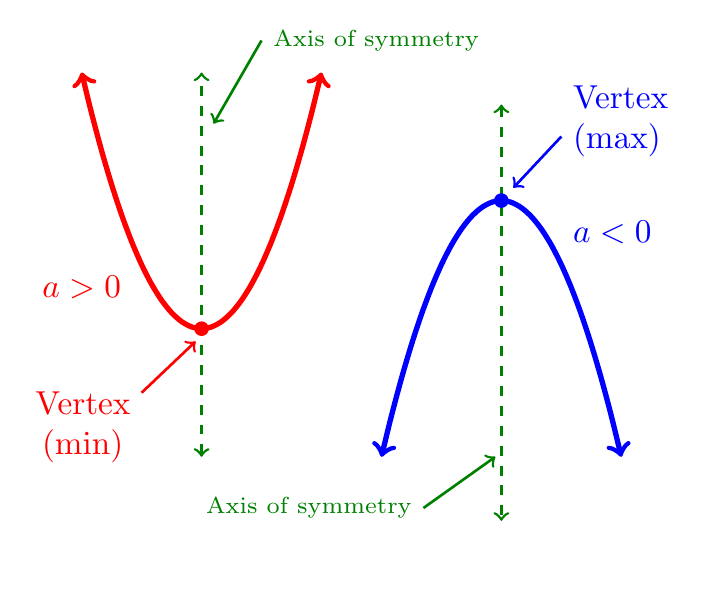
\begin{tikzpicture}[scale=1.2]
	\begin{axis}[axis line style={draw=none},
    ticks=none, tick style={draw=none}]
	\addplot[{<->},domain=-4:0,smooth, ultra thick, red] {(x+2)*(x+2)};
	\addplot[{<->},domain=1:5,smooth, ultra thick, blue] {-(x-3)*(x-3)+2};
	% dashe lines
	\addplot[{<->},dashed, thick, agreen] coordinates {(-2,-2)(-2,4)};
	\addplot[{<->},dashed, thick, agreen] coordinates {(3,3.5)(3,-3)};
	% a > 0
    \node [below, red] at (-4,1) {$a>0$};
    \node [below left, red,text width=1cm,align=center] at (-3,-0.8) {Vertex (min)};
    \addplot[mark=*,blue,red] coordinates {(-2,0)};
    \draw [->,thick,red] (-3,-1) -- (-2.1,-0.2);
    % a < 0
    \node [right, blue] at (4,1.5) {$a<0$};
    \draw [->,thick,blue] (4,3) -- (3.2,2.2);
    \node [above right, blue,text width=0.5cm,align=center] at (4,2.5) {Vertex (max)};
    \addplot[mark=*,blue] coordinates {(3,2)};
    %%%% axis of symmetry %%%%%
    \draw [->,thick,agreen] (-1,4.5) -- (-1.8,3.2);
    \node [right, agreen] at (-1,4.5) {\scriptsize Axis of symmetry};
    \draw [->,thick,agreen] (1.7,-2.8) -- (2.9,-2);
    \node [left, agreen] at (1.7,-2.8) {\scriptsize Axis of symmetry};
    \end{axis}
\end{tikzpicture}
\end{center}
\caption{Parabola opens upward if $a>0$ and open downward if $a<0$.}
\label{fig:parabola}
\end{figure}
%


As it is illustrated in Figure \ref{fig:parabola}:
\begin{enumerate}[1.]
    \item The graph opens upward (concave up) if $a>0$ and opens downward (concave down) when $a<0$.
    \item \textbf{The vertex (or turning point)} of a parabola is the lowest point on the graph when it open upward and the highest point when it opens downward.
    \item \textbf{The axis of symmetry} is a  vertical line through the vertex divides the figure in half.  Parabolas are symmetric with respect to this line.
\end{enumerate}
\section{Vertex}
Vertex is a very important point on a parabola. Not only it helps us to graph the parabola perfectly, but also it is a key point in optimization problems.\\
The quadratic functions can be written in either \textbf{standard form} or \textbf{general form}. Each form has its own way to find the vertex. Once we found the vertex, we can easily find the axis of symmetry.
\subsection{Standard form of a quadratic function}
The standard form of a quadratic function is 
\begin{equation}
            f(x) = a(x-h)^2+k
            \label{std_qdrt}
\end{equation}
The vertex of a standard quadratic function is located at $(h,k)$. This can be easily proven using the graph of standard function $y=x^2$ and transformation method.\\
The axis of symmetry is a vertical line passes through the vertex. Therefore, the equation of axis of symmetry of standard quadratic function is $x=h$.
% ====== EXAMPLE 1
\begin{exa}
    Find the vertex and axis of symmetry of the following functions.
    \begin{enumerate}[\bfseries a.]
        \item $f(x)= -(x-4)^2+3$
        \item $g(x)= 3(x+2)^2-1$
    \end{enumerate}
\end{exa}
%
a. Comparing the equation with \eqref{std_qdrt} equation, we get $h=4$ and $k=3$. Therefore, the vertex is located at $(4,3)$ and the axis of symmetry is $x=4$.\\[0.5cm]
%
b. First, rewrite the equation in standard form, 
\[
        g(x)=3\bigr(x-(-2)\bigl)^2-1
\]
Thus, $h=-2$ and $k=-1$ which gives us vertex $(-2,-1)$ and the axis of symmetry $x=-2$.
%================
\subsection{General form of a quadratic function}
We have already seen the general form of a quadratic function
\begin{equation}
            f(x) = ax^2+bx+c
            \label{gen_qdrt}
\end{equation}
The vertex of a quadratic function in this form is at $\biggl(-\frac{b}{2a}, f\bigr(-\frac{b}{2a}\bigl)\biggr)$. Therefore, the axis of symmetry is $x=-\frac{b}{2a}$.
% ======= EXAMPLE 2
\begin{exa}
    Find the vertex and the axis of symmetry of the following functions.
        \begin{enumerate}[\bfseries a.]
        \item $f(x)= -x^2+4x+2$
        \item $g(x)= 3x^2+x+10$
    \end{enumerate}
\end{exa}
%
a. Comparing with the general form, we got $a=-1$, $b=4$ and $c=2$, so the $x$-coordinate of vertex is 
\begin{align*}
    -\frac{b}{2a}&      &       &\text{Substitute}\\
    -\frac{4}{2(-1)}&   &       &\text{Simplify}\\
    2&      &           &\text{$x$-coordinate of the vertex}
\end{align*}
To find its $y$-coordinate, we need to plug $x=2$ into $f(x)$, therefore
\begin{align*}
    f(2)&     &   &\text{Plug it into function}\\
    -(2)^2+4(2)+2&  &   &\text{Simplify}\\
    6&      &       &\text{$y$-coordinate of the vertex}
\end{align*}
So the vertex is at $(2,6)$ and the axis of symmetry is $x=2$. \\[0.5cm]
%
b.Here we have $a=3$, $b=1$ and $c=10$, therefore the $x$-coordinate of the vertex is 
\[
            -\frac{b}{2a} =-\frac{1}{2(3)}=-\frac{1}{6}
            \]
And its $y$-coordinate is 
\[
            g\biggl(-\frac{1}{6}\biggr) = 3\biggl(-\frac{1}{6}\biggr)^2+\biggl(-\frac{1}{6}\biggr)+10 = \frac{119}{12}
\]
So the vertex is located at $\displaystyle \biggl(-\frac{1}{6},\, \frac{119}{12}\biggr)$. The axis of symmetry is simply $\displaystyle x=-\frac{1}{6}$.
% =============